\documentclass[12pt, letterpaper, preprint]{aastex}
\usepackage[breaklinks,colorlinks, urlcolor=blue,citecolor=blue,linkcolor=blue]{hyperref}
\usepackage{color}
\usepackage{amsmath}
\usepackage{natbib}
\usepackage{bm}
%%% This file is generated by the Makefile.
\newcommand{\giturl}{\url{https://github.com/changhoonhahn/nonGaussLike}}
\newcommand{\githash}{0cff07b}\newcommand{\gitdate}{2018-01-09}\newcommand{\gitauthor}{ChangHoon Hahn}


% typesetting shih
\linespread{1.08} % close to 10/13 spacing
\setlength{\parindent}{1.08\baselineskip} % Bringhurst
\setlength{\parskip}{0ex}
\let\oldbibliography\thebibliography % killin' me.
\renewcommand{\thebibliography}[1]{%
  \oldbibliography{#1}%
  \setlength{\itemsep}{0pt}%
  \setlength{\parsep}{0pt}%
  \setlength{\parskip}{0pt}%
  \setlength{\bibsep}{0ex}
  \raggedright
}
\setlength{\footnotesep}{0ex} % seriously?

% citation alias
\defcitealias{beutler2017}{B2017}
\defcitealias{sinha2017a}{S2017}

% math shih
\newcommand{\setof}[1]{\left\{{#1}\right\}}
\newcommand{\given}{\,|\,}
\newcommand{\pseudo}{{\mathrm{pseudo}}}
\newcommand{\Var}{\mathrm{Var}}
% text shih
\newcommand{\foreign}[1]{\textsl{#1}}
\newcommand{\etal}{\foreign{et~al.}}
\newcommand{\opcit}{\foreign{Op.~cit.}}
\newcommand{\documentname}{\textsl{Article}}
\newcommand{\equationname}{equation}
\newcommand{\bitem}{\begin{itemize}}
\newcommand{\eitem}{\end{itemize}}
\newcommand{\beq}{\begin{equation}}
\newcommand{\eeq}{\end{equation}}
\newcommand{\todo}[1]{{\bf \textcolor{red}{#1}}}
\newcommand{\Dmock}{\mathbf{D}^\mathrm{mock}}
\newcommand{\Xmock}{{\bf X}^\mathrm{mock}}
\newcommand{\Xref}{{\bf X}^\mathrm{ref}}
\newcommand{\Yref}{{\bf Y}^\mathrm{ref}}
\newcommand{\Ralpha}{R\'enyi-$\alpha$}
\newcommand{\Beut}{\citetalias{beutler2017}}
\newcommand{\Sinh}{\citetalias{sinha2017a}}

\newcommand{\patchy}{{\fontshape\scdefault\selectfont patchy}}

\begin{document}\sloppy\sloppypar\frenchspacing 

%\title{How I Learned to Stop Worrying and Love The Central Limit Theorem}
\title{Likelihood Non-Gaussianity in Large Scale Structure Analyses}
\date{\texttt{DRAFT~---~\githash~---~\gitdate~---~NOT READY FOR DISTRIBUTION}}
\author{ChangHoon~Hahn\refstepcounter{footnote}\refstepcounter{footnote}, et al.} %Florian~Beutler, Manodeep~Sinha, Andreas~Berlind}
\affil{Lawrence Berkeley National Laboratory, 1 Cyclotron Rd, Berkeley CA 94720, USA}
\email{changhoon.hahn@lbl.gov}

\begin{abstract}
    abstract here 
\end{abstract}

\keywords{
methods: statistical
---
galaxies: statistics
---
methods: data analysis
---
cosmological parameters
---
cosmology: observations
---
large-scale structure of universe
}

\section{Introduction}
\begin{itemize}
    \item Talk about the use of Bayesian parameter inference and getting the posterior in LSS cosmology 
    \item Explain the two major assumptions that go into evaluating the likelihood
    \item Emphasize that we are not talking about non-Gaussian contributions to the likelihood
    \item Emphasize the scope of this paper is to address whether one of the assumptions matters for 
        galaxy clustering analyses. 
\end{itemize}

% Data analysis can only lead to unbiased constraints on a physical theory if the employed likelihood is correct (e.g.  Trotta 2008; Mardia et al. 1979; Anderson 2003; Cramer 1946; Jeffreys 1961; Sun & Berger 2006). 
\begin{itemize}
    \item Depending on Hogg's paper maybe a simple illustration of how the likelihood asumption 
\end{itemize}

\todo{However, as we show in this paper, the assumption of likelihood 
Gaussianity is not necessary. In fact, we will show that the mock catalogs 
used in standard LSS analyses to estimate the covariance matrix for 
evaluating the Gaussian likelihood, can be used to quantify the non-Gaussianity. 
More important the mock catalogs can be used to construct an accurate 
estimator for the non-Gaussian likelihood.} 

\section{Mock Catalogs}
Mock catalogs play an indispensable role in standard cosmological 
anslyses of LSS studies. They're used for testing analysis 
pipelines~\citep[][]{beutler2017, grieb2017, tinkerinpreparation}, 
testing the effect of systematics~\citep{guo2012, vargas-magana2014, hahn2017, pinol2017, ross2017}, 
and, most relevantly for this paper, estimating the covariance 
matrix~\citep[][]{parkinson2012, kazin2014, grieb2017, alam2017, beutler2017, sinha2017a}. 
In fact, nearly all current state-of-the-art LSS analyses use
covariance matrices estimated from mocks to evaluate the likelihood 
for parameter inference. 

While some argue for analytic estimates of the covariance 
matrix~\citep[e.g.][]{mohammed2017} or estimates directly from data
by subsampling~\citep[e.g.][]{norberg2009}, covariance matrices 
from mocks have a number of advantages. Mocks allow us 
to incorporate detailed systematic errors present in the 
data and variance beyond the volume of the data. Even for analytic 
estimates, a large ensemble of mocks are crucial for validataion~\citep[\emph{e.g.}][]{slepian2017}. 
Moreover, as we show later in this paper, mocks present an
additional advantage: they allow us to 
quantify the non-Gaussianity of the likelihood and more accurately 
estimate the true likelihood distribution. 

In this paper, we we focus on two LSS analyses: the powerspectrum 
multipole ($P_\ell$) analysis of \Beut~and group multiplicity 
function ($\zeta$) analysis of \Sinh. Throughout the paper we will 
make extensive use of the mock catalogs used in these analyses. 
In this section, we give a brief description of these mocks and how 
the observables used in the analysis --- the powerspectrum 
multipole ($P_\ell$) and group multiplicity function ($\zeta(N)$) ---
are calculated from them. Afterwards, we will describe how we compute 
the covariance matrix from the mocks and pre-process the mock observable
data.

\subsection{MultiDark-PATCHY~Mock Catalog} \label{sec:patchy}
In their powerspectrum multipole analysis, \Beut~use 
the MultiDark-\patchy~mock catalogs from \cite{kitaura2016}. 
These mocks are generated using the \patchy~code \citep{kitaura2014,kitaura2015}. 
They rely on large-scale density fields generated using augmented
Lagrangian Perturbation Theory~\citep[ALPT;][]{kitaura2013} on a mesh,
which they then populate with galaxies based on a combined non-linear
deterministic and stochastic biases. The mocks from the \patchy~code 
are then calibrated to reproduce the galaxy clustering in the 
high-fidelity BigMultiDark $N$-body simulation~\citep{rodriguez-torres2016, klypin2016}. 
Afterwards, the galaxies are assigned stellar masses using the 
{\fontshape\scdefault\selectfont hadron}~code~\citep{zhao2015}.
and the {\fontshape\scdefault\selectfont sugar}~code~\citep{rodriguez-torres2016} 
is applied to combine different boxes, incorporate selection
effects and masking to produce mock light-cone galaxy catalogs. 
The statistics of the resulting mocks are then compared to 
observations and the process is iterated to reach desired 
accuracy. We refer readers to~\cite{kitaura2016} for further 
details. 

In total, \cite{kitaura2016} generated a 12,228 mock light-cone 
galaxy catalogs for BOSS Data Release 12. In \Beut, 
they use 2045 and 2048 for the northern galactic cap (NGC) and 
souther galactic cap (SGC) of the LOWZ+CMASS combined sample. 
\Beut~excluded 3 mock realizations due to notable 
issues, which have been since been addressed. Therefore, 
in our analysis we use all 2048 mocks for both the NGC and SGC of 
the LOWZ+CMASS combined sample.

\subsection{\cite{sinha2017a} Mocks} \label{sec:gmf} 
The simulations used in the small-scale clustering analysis of \cite{sinha2017a} 
are from the Large Suite of Dark Matter Simulations project~\citep[LasDamas;][]{mcbride2009} 
designed to model galaxy samples from SDSS DR7. They use initial conditions derived from 
second order Lagrangian Perturbation Theory using the 2LTPIC code~\citep{scoccimarro1998, crocce2006}
and evolved them using the $N$-body $\mathtt{GADGET}$-$2$ code~\citep{springel2005}.
Halos are then identified from the dark matter distribution outputs using 
the $\mathtt{ntropy-fofsv}$ code~\citep{gardner2007}, which uses a 
friend-of-friends algorithm~\citep[FoF;][]{davis1985} with a linking length of $0.2$
times the mean inter-particle separation. %The FoF halo masses are then adjusted using the \cite{warren2006} correction. 
\Sinh~uses two configurations of the LasDamas simulations.
The Consuelo simulation contains $1400^3$ dark matter particles with 
mass of $1.87 \times 10^9\,h^{-1} M_\odot$ in a cubic volume of 
$420\,h^{-1} Mpc$ per side evolved from $z_\mathrm{init} = 99$. 
The Carmen simulation contains $1120^3$ dark matter particles with mass 
of $4.938 \times 10^{10}\,h^{-1} M_\odot$ in a cubic volume of 
$1000\,h^{-1} Mpc$ per side evolved from $z_\mathrm{init} = 49$. 
%They use the following cosmological parameters, which are motivated by the WMAP3 constraints \citep{spergel2007}: $\Omega_m = 0.25, \Omega_\Lambda = 0.75, \Omega_b = 0.04, h = 0.7, \sigma_8 = 0.8,\;\mathrm{and}\;n_s = 1.0.$

The FoF halo catalogs are then populated with galaxies using the 
`Halo Occupation Distribution` (HOD) framework. The 
number, positions, and velocities of galaxies are described statistically 
by an HOD model. \Sinh~adopts the `vanilla' HOD model of \cite{zheng2007}, 
where the mean number of central and satellite galaxies are described by 
the halo mass and five HOD parameters: $M_\mathrm{min}, 
\sigma_{\log\,M} , M_0, M_1,~\mathrm{and}~\alpha$. Lastly, once the 
simulation boxes are populated with galaxies, observational systematic 
effects are imposed. The peculiar velocities of galaxies are used to 
impose redshift-space distortions. Galaxies that lie outside the redshift
limits or sky footprint of the SDSS sample are removed. For further 
details regarding the mocks, we refer readers to \Sinh.

To calculate their covariance matrix, \Sinh~produced 200 
independent mock catalogs from 50 simulations using a single set of 
HOD model parameters. To take advantage of the methods we later 
present (Sections~\ref{sec:gmm} and~\ref{sec:ica}), we require a large 
number of mocks. Our methods rely on using the mocks to sample high 
dimensional distributions, so incorporating more mocks improves their 
accuracy. We utilize an addition $99$ sets of HOD parameters with $200$
mocks each. These parameters are sampled from the MCMC chain used to 
produce the posterior in~\Sinh. In total we use $20,000$ mocks. 

\subsection{Mock Observable ${\bf X}^\mathrm{mock}$ and Covariance Matrix $\mathbb{C}$} \label{sec:xmock}
To get from the mock catalogs described above to the covariance matrices 
used in~\Beut~and~\Sinh, the observables are measured for each mock in 
the \emph{same} way as the observations. We briefly describe how $P_\ell(k)$ and $\zeta(N)$ 
and their covariance matrices are measured in \Beut~and \Sinh. We then 
describe how we pre-process the mock observables for the methods we describe 
in the next sections.

To measure the powerspectrum multipoles of the BOSS DR12 galaxies
and the MutliDark-\patchy~mocks (Section~\ref{sec:patchy}), \Beut~uses a 
fast fourier transform (FFT) based anisotropic powerspectrum estimator 
based on \cite{bianchi2015} and \cite{scoccimarro2015}. This estimator 
estimates the  monopole, quadrupole, and hexadecapole 
($\ell = 0, 2,\,\mathrm{and}\,4$) of the powerspectrum using FFTs of the 
overdensity field multipoles for a given survey geometry. For further 
details on the estimator we refer readers to~\Beut~Section 3. \Beut~compute
the powerspectrum over the range $k = 0.01 - 0.15\, h\,\mathrm{Mpc}^{-1}$
for $\ell = 0,\,\mathrm{and}\,2$ and $k = 0.01 - 0.10\, h\,\mathrm{Mpc}^{-1}$.
for $\ell = 4$. The powerspectrum multipoles are calculated in bins of 
$\Delta k = 0.01\,h\,\mathrm{Mpc}^{-1}$.

From the $\vec{P}^{(n)} = \big[P^{(n)}_{0}(k), P^{(n)}_{2}(k), P^{(n)}_{4}(k) \big]$ 
of the MultiDark-\patchy~mocks, \Beut~computes the $(i, j)$ element of the 
covariance matrix of all multipoles as 
\beq
\mathbb{C}_{i,j} = \frac{1}{N_\mathrm{mock} - 1} \sum\limits_{n=1}^{N_\mathrm{mock}} \big[ \vec{P}^{(n)}_i - \overline{P}_i \big]
    \times \big[ \vec{P}^{(n)}_j - \overline{P}_j \big].
\eeq
$N_\mathrm{mock} = 2048$ is the number of mocks and $\overline{P}_i$ is the mean 
of the mock powerspectra: $\overline{P}_i = \frac{1}{N_\mathrm{mock}} \sum_{n=1}^{N_\mathrm{mock}} \vec{P}^{(n)}_i$.
Since $P_0$ and $P_2$ each have $14$ bins and $P_4$ has $9$ bins, 
$\mathbb{C}$ is a $37 \times 37$ matrix.
In this work, we compute the $P_\ell(k)$ using a similar FFT-based 
estimator of \cite{hand2017a} instead of the~\Beut~estimator. Our choice 
is based on computational convenience. A python implementation
of the \cite{hand2017a} estimator is publicly available in the $\mathtt{NBODYKIT}$ 
package\footnote{http://nbodykit.readthedocs.io/en/latest/index.html}. 
We confirm that the resulting $P_\ell(k)s$ and covariance matrices from 
the two estimators are consistent with one another. 

Next, for the \Sinh~group multiplicity function analysis, they start 
with the \cite{berlind2006} FoF algorithm to identify groups in the 
SDSS and mock data. \Sinh~adopts the \cite{berlind2006} linking lengths
in units of mean inter-galaxy separation: $b_\perp = 0.14$ and $b_\parallel = 0.75$.
In comoving lengths, the linking lengths for the SDSS DR7 $M_r < -19$ 
sample correspond to $(r_\perp, r_\parallel) = (0.57, 3.05)h^{-1}\,\mathrm{Mpc}$. 
Once the groups are identified in the SDSS and mock data, $\zeta(N)$
is derived by calculating the comoving number density of groups 
in bins of richness $N$ --- the number of galaxies in the group. 
For the $M_r < −19$ SDSS sample, \Sinh~uses eight $N$ bins: 
$(5 - 6), (7 - 9), (10 - 13), (14 - 19), (20 - 32), (33 - 52), (53 - 84), (85 - 220)$.
For further details on the GMF calculation, we refer readers to 
\Sinh~Section 4.2.  
From the $\zeta^{(n)}(N)s$ of each mock, \Sinh~computes the $(i, j)$ element of
the covariance matrix as 
\beq \label{eq:gmf_cov} 
\mathbb{C}_{i,j} = \frac{1}{N_\mathrm{mock} -1} \sum\limits_{n=1}^{N_\mathrm{mock}} \big[\zeta^{(n)}(N_i) -  \bar{\zeta}(N_i)\big] \times
    \big[\zeta^{(n)}(N_j) -  \bar{\zeta}(N_j)\big].
\eeq
In \Sinh, they compute the covariance matrix using $200$ mocks
generated using a single fiducial set of HOD parameters. As we 
describe in Section~\ref{sec:gmf}, in this paper we use $20,000$ mocks from 
$100$ different set of HOD parameters sampled from the MCMC chain. 
The GMF covariance matrix we use in this paper is computed with 
$N_\mathrm{mock} = 20,000$ mocks. 

For the rest of the paper, in order to discuss the two separate 
analyses of~\Beut~and~\Sinh~in a consistent manner, we define the matrix 
$\Dmock$ of the mock observables ($P_\ell$ and $\zeta$) as 
\beq
\Dmock = \Big\{{\bf D}^\mathrm{mock}_n \Big\} \quad\quad \mathrm{where}\,\,\Dmock_n
\begin{cases}
    \vec{P}^{(n)} &\quad\mathrm{for}\,\, \mathrm{B}2017,\\ 
    \zeta^{(n)} &\quad\mathrm{for}\,\, \mathrm{S}2017.
\end{cases} 
\eeq
$\Dmock$ has dimensions of $2048 \times 37$ and $20,000\times8$ 
for \Beut~and \Sinh~respectively. 

For the methods in Sections~\ref{sec:gmm}~and~\ref{sec:ica}, the mock 
observable data ($\Dmock$) need to be pre-processed. \todo{why preprocess}
This pre-processing
involves two steps: mean-subtraction and whitening. For mean subtraction, 
the mean of the observable is subtracted from $\Dmock$. Then 
$\Dmock - \overline{\bf D}^\mathrm{mock}$ is whitened using a linear transformation 
to remove the Gaussian correlation between the bins of $\Dmock$: 
\beq
\Xmock = L\,(\Dmock - \bar{\bf D}^\mathrm{mock}). 
\eeq
The linear transformation is derived so that covariance matrix of the whitened 
data, $\Xmock$, is the identity matrix $\mathbb{I}$. Such a whitening linear 
transformation can be derived in infinite ways. 
One way to derive the linear transformation is through the eigen-decomposition
of the covariance matrix~\citep[\emph{e.g.}][]{hartlap2009, sellentin2017}. We, alternatively, 
derive the linear transformation ${\bf L}$ using Choletsky decompositon of the 
inverse covariance matrix~\citep{Press:1992:NRC:148286}: 
$\mathbb{C}^{-1} = {\bf L}\,{\bf L}^T$. \todo{We confirm tha the different 
whitening algorithms, does not impact the results of the paper.}
Now that we have the pre-processed data of the mock observables, 
we proceed in the next section to quantifying the non-Gaussianity of the 
$P_\ell$ and $\zeta$ likelihoods. 


\section{Quantifying the Likelihood non-Gaussianity} \label{sec:div}
The standard approach to parameter inference in LSS studies neglects
to account for likelihood non-Gaussianity. 
However, we are not the first to investigate likelihood non-Gaussianity 
in LSS analyses. Nearly two decades ago, \cite{scoccimarro2000} examined 
the likelihood non-Gaussianity for the powerspectrum and reduced bispectrum 
using mock catalogs of the IRAS redshift catalogs. More recently, 
\cite{hartlap2009} and \cite{sellentin2017} examined the non-Gaussianity 
of the cosmic shear correlation function likelihood using simulations of 
the Chandra Deep Field South and CFHTLenS, respectively. 

While these works present different methods for identifying 
likelihood non-Gaussianity, they do not present a concrete way of 
quantifying it. \cite{hartlap2009}, for instance, identifies the
non-Gaussianity of the cosmic shear likelihood by looking at the
statistical independence/dependence of PCA components of the mock 
observable. In \cite{sellentin2017}, they use the Mean
Integrated Squared Error (MISE) as a distance metric between 
Gaussian random variables and the whitened mock observable 
data vector to characterize non-Gaussian correlations between elements 
of the data vector. These indirect measures of likelihood non-Gaussianity 
are challenging to interpret and extend more generally to LSS studies. 
%Sellentin & Heavens (2018) presented stringent tests that characterize non-Gaussian statistical behaviour, and any sound weak lensing likelihood should hence pass these tests.  The methods derived in Sellentin & Heavens (2018) test whether all pairwise combinations of data elements display the correct statistical behaviour under addition, division and multiplication, and whether the correct marginal distribution ensues for each data point. 

A more direct approach, however, can be taken to quantify the 
non-Gaussianity of the likelihood. We can calculate the divergence between 
the distribution of our observable, $p(x)$, and $q(x)$ a multivariate Gaussian described 
by the average of the mocks and the covariance matrix.
The following are two of the most commonly used divergences: 
the Kullback-Leibler (KL) divergence
\beq \label{eq:kl} 
D_{KL} ( p \parallel q ) = \int p(x)\,\log \frac{p(x)}{q(x)}\,{\rm d}x
\eeq
and the R\'enyi-$\alpha$ divergence
\beq \label{eq:renyi}
D_{R-\alpha} ( p \parallel q ) = \frac{1}{\alpha -1} \log \int p^\alpha(x)\, q^{1 -\alpha}(x)\,{\rm d}x. 
\eeq
In the limit as $\alpha$ approaches 1, the R\'enyi-$\alpha$ divergence is
equivalent to the KL divergence.
%To evaluate the R\'enyi-$\alpha$ divergence, we need to evaluate the following
%kernel function
%\beq \label{eq:d_alpha}
%D_{\alpha} ( p \parallel q ) = \int p^\alpha(x) q^{1-\alpha}(x)\,{\rm d}x. 
%\eeq

Of course, in our case, we don't know $p(x)$ --- \emph{i.e.} the distribution of
our observable. If we did, we would simply use that instead of bothering with 
the covariance matrix or this paper. We can, however, still estimate the 
divergence using nonparametric divergence estimators~\citep{wang2009, poczos2012, krishnamurthy2014}. 
These estimators allow us to estimate the divergence directly from 
samples $X_{1:n} = \{ X_1, ... X_n \}$ and $Y_{1:m} = \{ Y_1, ... Y_m \}$ 
drawn from $p$ and $q$ respectively: $\hat{D}_{\alpha}(X_{1:n} \parallel Y_{1:m})$. 
For instance, the estimator presented in \cite{poczos2012} allows us to estimate 
the kernel function of the R\'enyi-$\alpha$ divergence,
\beq \label{eq:d_alpha}
D_{\alpha} ( p \parallel q ) = \int p^\alpha(x) q^{1-\alpha}(x)\,{\rm d}x. 
\eeq
using $k^\mathrm{th}$ nearest neighbor density estimators. Let $\rho_k(x)$ 
denote the Euclidean distance of the $k^\mathrm{th}$ nearest neighbor 
of $x$ in the sample $X_{1:n}$ and $\nu_k(x)$ denote the Euclidean distance 
of the $k^\mathrm{th}$ nearest neighbor of $x$ in the sample $Y_{1:m}$. Then 
\beq \label{eq:d_alpha_est}
D_{\alpha}(p \parallel q) \approx \hat{D}_{\alpha}(X_{1:n} \parallel Y_{1:m}) = \frac{B_{k,\alpha}}{n} \left(\frac{n-1}{m}\right)^{1-\alpha}
\sum\limits_{i=1}^{n} \left(\frac{\rho_k^{d}(X_i)}{\nu_k^{d}(X_i)} \right)^{1-\alpha},
\eeq
where $B_{k, \alpha} = \frac{\Gamma(k)^2}{\Gamma(k-\alpha+1)\Gamma(k+\alpha-1)}$. 
This estimator, as \cite{poczos2012} proves, is asymptotically unbias,
\beq
\lim_{n, m \rightarrow \infty} \mathbb{E} \big[ \hat{D}_{\alpha} (X_{1:n} \parallel Y_{1:m}) \big] = D_{\alpha} (p \parallel q).
\eeq
Plugging $\hat{D}_{\alpha}(X_{1:n} \parallel Y_{1:m})$ into Eq.~\ref{eq:renyi},
we get an estimator for the R\'enyi-$\alpha$ divergence. \cite{wang2009} dervies
a similar estimator for the KL divergence~(Eq.~\ref{eq:kl}). 
%We note that while the divergence estimators converge to the true divergence with a large enough samples, with a limited number of samples from the distribution, the estimators are noisy. 

These divergence estimates have been applied to Support Vector Machines and used 
extensively in the machine learning and astronomical literature with great success 
\todo{elaborate a lot more} 
\bitem 
    \item Compile papers that use this divergence, \cite{ntampaka2015, ntampaka2016}
\eitem
For more details on the non-parametric divergence estimators, we refer readers to 
\cite{poczos2012} and \cite{krishnamurthy2014}.

With these estimators, we can now explicitly quantify the 
non-Gaussianity of the likelihood by computing the divergence 
between the likelihood distribution and the Gaussian 
pseudo-likelihood distribution:
$D(\, p(x) \parallel \mathcal{N}(\overline{\bf X}^\mathrm{mock}, \mathbb{C}\,))$. 
We draw a reference sample ${\bf Y}^\mathrm{ref}$ from 
$\mathcal{N}(\overline{\bf X}^\mathrm{mock}, \mathbb{C})$ then 
since $\Xmock$ is in principle sampled from $p(x)$, we can use the 
estimators to compute $\hat{D}(\Xmock \parallel \mathcal{N})$.
Similar to the experiments detailed in \cite{poczos2012}, 
we construct ${\bf Y}^\mathrm{ref}$ with a comparable sample size as $\Xmock$: 
$2000$ and $10,000$ for the $P_\ell$ and $\zeta$ analyses respectively. 

In Figure~\ref{fig:div_gauss}, we present the resulting \Ralpha~(left) 
and KL (right) divergences ($\hat{D}_{R\alpha}$ and $\hat{D}_{KL}$; orange) 
for the \Beut~$P_\ell$ (top) and \Sinh~$\zeta$ (bottom) analyses.
As a reference for comparison, we also include in blue divergence 
estimates of the pseudo-likelihood onto itself, which we calculate as 
$\hat{D}(\Xref \parallel \Yref)$. $\Xref$ is a data vector with 
the same dimension as $\Xmock$ sampled from the pseudo-likelihood 
$\mathcal{N}$. Since $\hat{D}$ are estimates, rather than the true divergence, 
we compute each of the estimates \todo{100} times (resampling 
$\Yref$ each time) and present their distribution in order to 
illustrate their uncertainty.
Each panel of Figure~\ref{fig:div_gauss} show significant 
discrepancy between the two distributions. This suggests that both 
the $P_\ell(k)$ and $\zeta(N)$ likelihoods are \emph{significantly 
non-Gaussian}. 
%In more detail, we see that the $\zeta(N)$ likelihood is significantly more non-Gaussian than the $P_\ell(k)$ likelihood. 

%%%%%%%%%%%%%%%%%%%%%%%%%%%%%%%%%%%%%
% Figure 1 
%%%%%%%%%%%%%%%%%%%%%%%%%%%%%%%%%%%%%
\begin{figure}
\begin{center}
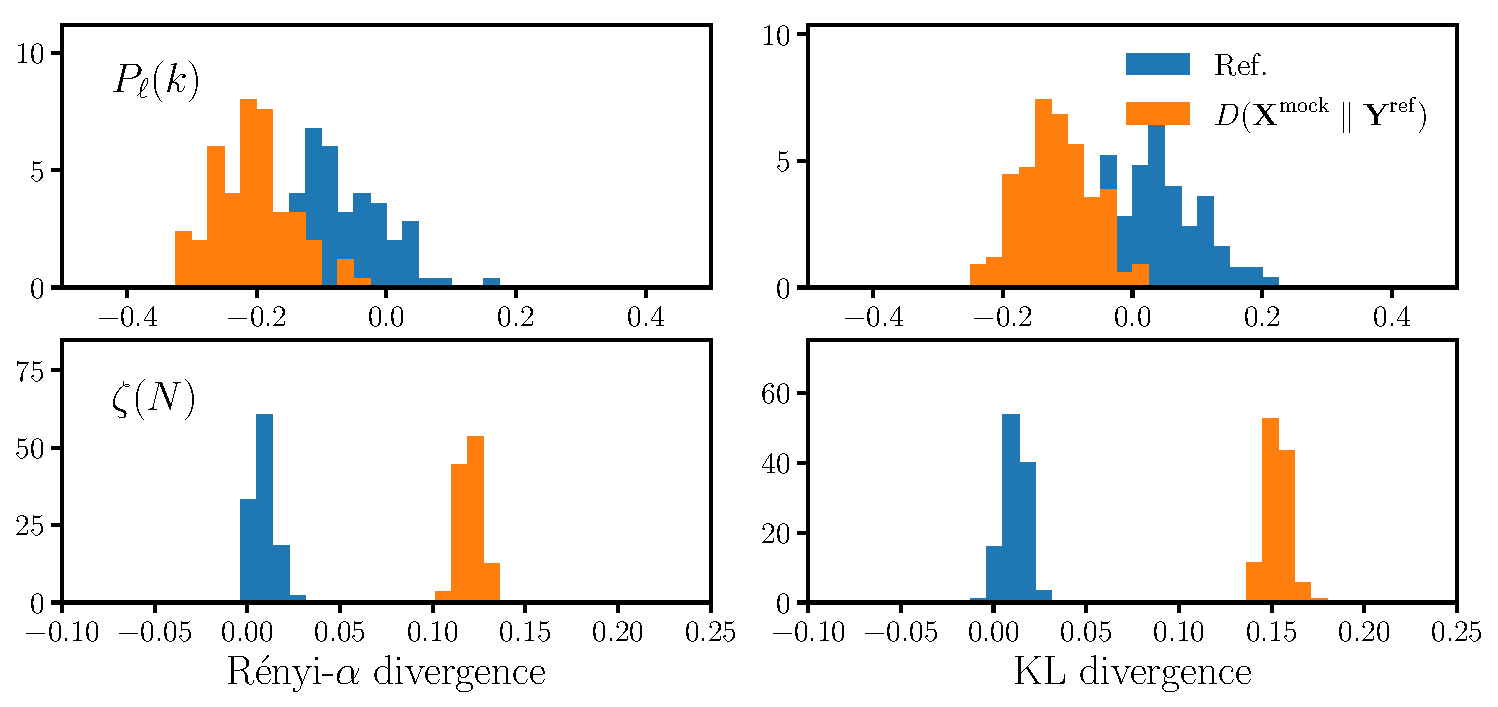
\includegraphics[width=0.9\textwidth]{figs/kNNdiverg_Gauss.pdf}
    \caption{R\'enyi-$\alpha$ and KL divergence estimates 
    ($\hat{D}_{R\alpha}$ and $\hat{D}_{KL}$; orange) between 
    the likelihood distribution and the Gaussian pseudo-likelihood 
    for the \Beut~$P_\ell$ (top) and \Sinh~$\zeta$ (bottom) analyses. 
    We include in blue, as reference, the divergence estimates 
    of the pseudo-liklihood onto itself.  
    $\hat{D}_{R\alpha}$ and $\hat{D}_{KL}$ are computed using the 
    non-parametric $k$-NN estimator (Section~\ref{sec:div}) on 
    the mock data $\Xmock$ and a referece sample $\Yref$ drawn
    from the pseudo-likelihood. We compute $\hat{D}_{R\alpha}$ and
    $\hat{D}_{KL}$ \todo{100} times and plot their distribution 
    in order to illustrate the uncertainty in the $\hat{D}$ 
    estimator. The significant discrepancy between 
    the two divergence distributions in each of the panels, identifies 
    the \emph{significant non-Gaussianity of the $P_\ell(k)$ and $\zeta(N)$ 
    likelihoods}. 
    }
\label{fig:div_gauss}
\end{center}
\end{figure}
%%%%%%%%%%%%%%%%%%%%%%%%%%%%%%%%%%%%%

\section{Estimating the Non-Gaussian Likelihood}
In the previous section, we estimate the divergence between the 
$P_\ell$ and $\zeta$ likelihoods sampled by mocks and their respective 
Gaussian pseudo-likelihoods. These divergences identify and quantify 
the significant non-Gaussianity in the likelihoods of LSS studies.   
Our ultimate goal, however, is to quantify the impact of likelihod 
non-Gaussianity on the final cosmological parameter constrains and
to develop more accurate methods for parameter inference in LSS. 
From the divergence estimates alone, it's not obvious how they propagate 
onto the final parameter constraints. Therefore in this section, 
we present two methods for more accurately estimating the non-Gaussian 
likelihoods of $P_\ell$ and $\zeta$ from the corresponding mocks.
These methods provide a more accurate estmiate of the likelihood than 
the Gaussian pseudo-likelihood. Moreover, we will use them later to 
quantify the impact of likelihood non-Gaussianity on the 
\Beut~and \Sinh~parameter constraints. 

\subsection{Gaussian Mixture Likelihood Estimation} \label{sec:gmm}
When mock catalogs are used for parameter inference in LSS analyses, 
they essentialy serve as data points sampling the likelihood distribution. 
For the pseudo-likelihood, this distribution is assumed to have a 
Gaussian functional form. Hence, why we estimate the covariance matrix 
from mocks. However, the Gaussian functional form, or any functional form for 
that matter, is \emph{not} necessary to estimate the likelihood distribution. 
Instead, the multidimensional likelihood distribution 
can be directly estimated from the set of mock catalogs using --- for 
instance using Gaussian mixture density estimation~\citep{9780471006268}. 
\todo{talk about how this is used extensively in ML} 
In astronomy, Gaussian mixture density estimation has been used for 
inferring the velocity distribution of stars from the Hipparcos 
satellite~\citep{bovy2011}, classifying galaxies in the Galaxy And Mass Assembly 
Survey~\citep{taylor2015}, and classifying pulsars~(\citealt{lee2012}; see
also references in \citealt{kuhn2017}). 

Gaussian mixutre density estimation is a ``semi-parametric'' method 
that uses a weighted sum of $k$ Gaussian component densities, a Gaussian 
mixture model (hereafter GMM)
\beq
p(x; \bm{\theta}) = \sum\limits_{i=1}^{k} \pi_i\, \mathcal{N}(x; \bm{\theta}_i),
\eeq
to estimate the density. 
The component weights ($\pi_i$; also known as mixing weights) and the 
component parameters $\bm{\theta}_i$ are free parameters of the mixture 
model. Given some data set ${\bf X}_N = \{{\bf x}_1,..., {\bf x}_N \}$, 
these free GMM parameters are, most popularly, estimated 
through an expectation-maximization algorithm~\citep[EM;][]{dempster1977, neal1998}.
The EM algorithm begins by randomly assigning $\bm{\theta}^0_i$ to the 
$k$ Gaussian components. The algorithm then iterates between two steps. 
In the first step, the algorithm computes for each data point, ${\bf x}_n$, 
a probability of being generated by each component of the model. These 
probabilities can be thought of as weighted assignments of the points 
to the components. Next, given the ${\bf x}_n$ assignment to the 
components, $\bm{\theta}^t_i$ of each component are updated to $\bm{\theta}^{t+1}_i$
to maximize the likelihood of the assigned points. At this point, $\pi_i$ 
can also be updated by summing up the assignment weights and 
normalizing it by the total number of data points, $N$. This entire
process is repeated until convergence --- \emph{i.e.} when the log-likelihood of 
given the mixture model $\log\,p({\bf X}_N; \bm{\theta}^t)$ %= \sum\limits_{n=1}^{N} \log\,p({\bf x}_n; \bm{\theta}^t)
converges. The EM algorithm is guaranteed to converges to a local maximum 
of the likelihood~\citep{wu1983}. 

In practice, instead of arbitrarily assigning the initial condition, 
$\bm{\theta}^0_i$ is derived from a $\mathtt{k}$-$\mathtt{means}$ 
clustering algorithm~\citep{lloyd1982}. Without going into details, the 
$\mathtt{k}$-$\mathtt{means}$ algorithm clusters the data ${\bf X}_N$ into $k$ 
clusters, each described by the mean (or centroid) $\mu_i$ of the
samples in the cluster. The algorithm then iteratively chooses centroids that 
minimize the average squared distance between points in the same cluster.
For our GMMs, we set the initialize the EM algorithm using 
the $\mathtt{k}$-$\mathtt{means}{\tiny ++}$ algorithm of ~\cite{arthur2007}. 
In Figure~\ref{fig:gmm_ped}, we illustrate Gaussian mixture 
density estimation in action. We use GMMs with $k = 1$ (top), $
3$ (middle), and $10$ (bottom) components to estimate the
distribution of one dimensional data (blue) drawn from three 
separate Gaussia distributions. The GMM outputs of the EM algorithm 
are plotted in red with dotted black lines representing each of their 
components.  

%%%%%%%%%%%%%%%%%%%%%%%%%%%%%%%%%%%%%
% Figure 2 
%%%%%%%%%%%%%%%%%%%%%%%%%%%%%%%%%%%%%
\begin{figure}
\begin{center}
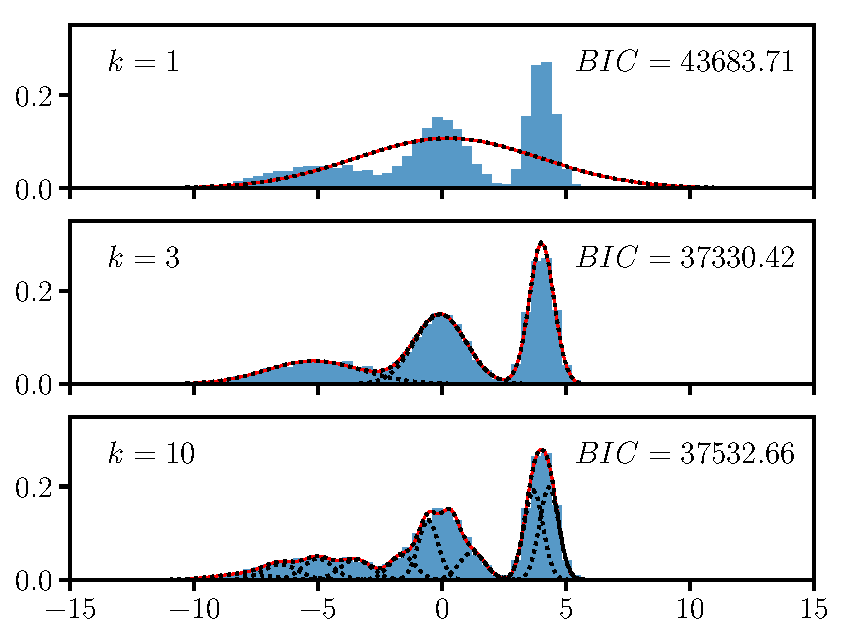
\includegraphics[width=0.75\textwidth]{figs/GMM_pedagog.pdf}
\caption{A pedagogical illustration of Gaussian mixture density estimation.
    We use GMMs with $k = 1$ (top), $3$ (middle), $10$ (bottom) 
    components to estimate the distribution of data (blue) drawn from three 
    Gaussian distributions. The GMM outputs of the EM algorithm 
    are plotted in red with \todo{dotted lines} representing each of their 
    components (Section~\ref{sec:gmm}). We also include the BIC of 
    the GMMs, which we use to select the number of components $k$. 
    Of the three panels, $k=3$ has the lowest BIC and therefore 
    best represents the data according to our selection scheme.} 
\label{fig:gmm_ped}
\end{center}
\end{figure}
%%%%%%%%%%%%%%%%%%%%%%%%%%%%%%%%%%%%%

So far in our description of GMMs, we have kept
the number of componenets $k$ fixed. However, $k$ is a free 
parameter and selecting it is a crucial step in Gaussian mixture
density estimation. With too many components the model may overfit 
the data; with too few components, 
the model may not be flexible enough to approximate the true 
underlying distribution. In order to address this model selection problem
of selecting $k$, we make use of the Bayesian Information 
Criterion~\citep[BIC;][]{schwarz1978}. BIC has been widely used for 
determining the number of components in mixture 
modeling~\citep[\emph{e.g.}][]{leroux1992,roeder1997,fraley1998,steele2010performance}
and for model selection in general in 
astronomy~\citep[\emph{e.g.}][]{liddle2007,broderick2011,wilkinson2015,vakili2016}.
According to BIC, models with higher likelihood are preferred; however, 
to address the concern of overfitting, BIC introduces a \emph{penalty} term 
for the number of parameters in the model: 
\beq \label{eq:bic}
\mathrm{BIC} = -2\,\mathrm{ln}\,\mathcal{L} + N_\mathrm{par}\,\mathrm{ln}N_\mathrm{data}.
\eeq
We select $k$ based on the number of components in the model with the 
lowest BIC. Of the three panels in Figure~\ref{fig:gmm_ped}, the GMM 
model with $k=3$ components has the lowest BIC and therefore would be 
selected. At least in this example, the choice of $k=3$ is 
obviously justified. The $k = 1$ GMM is definitely not flexible enough 
to characterize the underlying distribution and the $k=10$ GMM clearly
overfits the distribution. 

With Gaussian mixture density estimation we can directly estimate 
the likelihood distribution using the mock catalogs. We first fit 
GMMs with $k\mathrm{s} < 30$ components to the whitened 
mock data $\Xmock$ using the EM algorithm for each model. For each of the 
coverged GMMs, we calculate the BIC. Afterwards we select 
the model with the lowest BIC as the best density estimate of the likelihood 
distribution: $\hat{p}_\mathrm{\tiny GMM}(x)$. The selected density estimate can 
then be used to calculate the
likelihood and quantify the impact of likelihood non-Gaussianity on the 
parameter constraints of~\Beut~and~\Sinh. But before we do that, we have to 
confirm whether $\hat{p}_\mathrm{\tiny GMM}$ is in fact a better estimate 
of the likelihood over the Gaussian pseudo-likelihood. To do this, we return 
to the divergence estimates of Section~\ref{sec:div}. 

To estimate the divergence between our Gaussian mixture density estimate,
$\hat{p}_\mathrm{\tiny GMM}$, and the likelihood distribution, we take 
the same approach as our $\hat{D}$ calculation in Section~\ref{sec:div}. 
Instead of $\Yref$ drawn from the pseudo-likelihood, we draw 
samples from $\hat{p}_\mathrm{\tiny GMM}(x)$ with the same 
dimensions. Then we calculate $k$-NN~\Ralpha~and KL 
divergence estimates between this sample and $\Xmock$. As we did in Figure~\ref{fig:div_gauss}, 
we repreat this process \todo{100} times, resampling $\hat{p}_\mathrm{\tiny GMM}$
each time, in order get a distribution of divergence estimates that 
reflects the scatter in the estimator. In Figure~\ref{fig:div_gmm}, 
we present the resulting distribution of divergences between 
$\hat{p}_\mathrm{\tiny GMM}$ and the likelihood distribution in \todo{green} 
for the $P_\ell(k)$ (top) and $\zeta(N)$ (bottom) analyses. For comparison, 
we include the distributions from Figure~\ref{fig:div_gauss}. 

For the $\zeta(N)$ analysis of \Sinh, our Gaussian mixture density 
estimate significantly improves the divergence discrepancy compared to the 
pseudo-likelihood. In other words, \emph{our Gaussian mixture density estimate  
is a significant better estimate of the $\zeta$ likelihood distribution
than the pseudo-likelihood}. On the other hand, our Gaussian mixture 
density estimate for the $P_\ell(k)$ analysis of \Beut~does not 
significantly improve the divergence discrepancy. This difference in 
the performance of Gaussian mixture density estimation is not surprising. 
One would expect a direct density estimation to be more effective 
for the \Sinh~case, where we estimate an $8$-dimensional 
distribution with $N_\mathrm{mock} = 20,000$ samples, compared to the \Beut~ 
case where we estimate a $37$-dimensional distribution with 
only $N_\mathrm{mock} = 2048$ samples. 
Given the unconvincing accuracy of the Gaussian mixture density estimate
of the $P_\ell$ likelihood, in the next section we present an alterative 
method for estimating the non-Gaussian likelihood.

%%%%%%%%%%%%%%%%%%%%%%%%%%%%%%%%%%%%%
% Figure 3 
%%%%%%%%%%%%%%%%%%%%%%%%%%%%%%%%%%%%%
\begin{figure}
\begin{center}
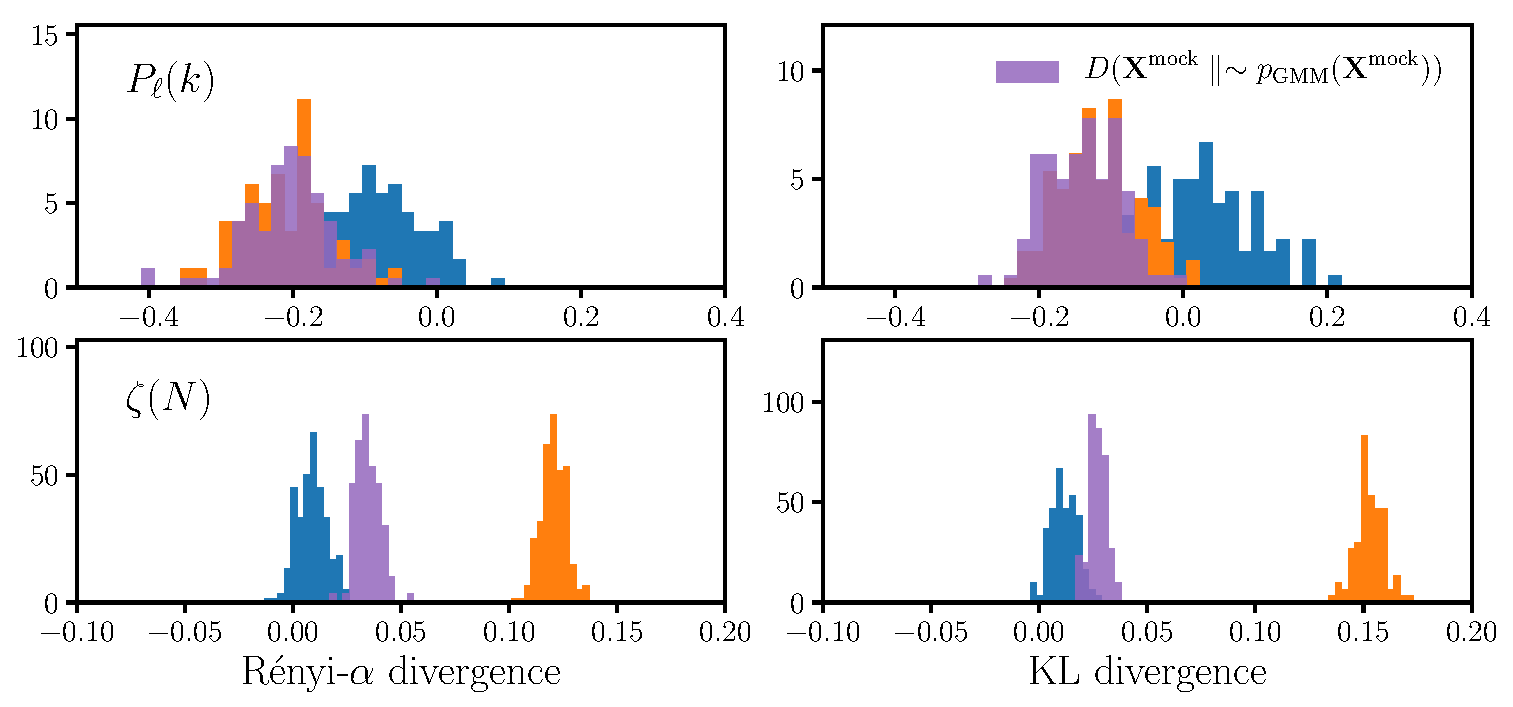
\includegraphics[width=0.9\textwidth]{figs/kNNdiverg_gmm.pdf}
\caption{R\'enyi-$\alpha$ and KL divergence estimates 
    ($\hat{D}_{R\alpha}$ and $\hat{D}_{KL}$; \todo{green}) between 
    the likelihood distribution and the Section~\ref{sec:gmm} GMM 
    likelihood estimate for the \Beut~$P_\ell$ (top) and \Sinh~$\zeta$ 
    (bottom) analyses. We include the divergence estimates from 
    Figure~\ref{fig:div_gauss} for comparison. The Gaussian mixture
    likelihood does not significantly improve the discrepancy in 
    divergence for the $P_\ell$ analysis. This is due to the high-dimensionality 
    (37 dimensions) of the $P_\ell$ likelihood. However, for the $\zeta$ 
    analysis, \emph{our Gaussian mixture likelihood estimate is 
    a significantly better estimate of the likelihood
    than the pseudo-likelihood.}
    }
\label{fig:div_gmm}
\end{center}
\end{figure}
%%%%%%%%%%%%%%%%%%%%%%%%%%%%%%%%%%%%%

\subsection{Independent Component Analysis} \label{sec:ica}
Gaussian mixture density estimation fails to accurately estimate 
the $37$-dimensional $P_\ell$ likelihood distribution of \Beut. 
Rather than estimating the likelihood distribution directly, 
if we can transform the observable ${\bf x}$ (\emph{e.g.} $P_\ell$) 
into statistically independent components ${\bf x}^\mathrm{IC}$ 
the problem becomes considerably simpler. Since ${\bf x}^\mathrm{IC}$ 
is statistically independent the likelihood distribution becomes 
\beq \label{eq:ica_like}
p(x) = \prod\limits_{n=1}^{N_\mathrm{bin}} p_{x^\mathrm{ICA}_n} (x) 
\eeq
where $N_\mathrm{bin}$ is the number of bins in the observable. 
For the \Beut~case, this reduces the problem of estimating a 37 
dimensional distribution with $2048$ samples to a problem of 
estimating 37 one dimensional distributions with $2048$ samples 
each. The challenge, however, is in finding the transformation ${\bf M}$. 

Efforts in the past have attempted to tackle this sort of 
high-dimensional problem~\citep[\emph{e.g.}][]{scoccimarro2000,eisenstein2001,gaztanaga2005,norberg2009,sinha2017a}.
They typically use singular value decomposition or principal 
component analysis~\citep[PCA;][]{Press:1992:NRC:148286}. For a Gaussian
likelihood, the PCA components of it are statistically independent. 
However, when the likelihood is \emph{not} Gaussian, the PCA components 
are uncorrelated but~\emph{not necessarily statistically independent}~\citep{hartlap2009}. 
Since the $P_\ell$ and $\zeta$ likelihoods are non-Gaussian, we cannot 
use PCA. Instead, we use Independent Component Analysis (ICA) following 
\cite{hartlap2009}. 

In order to find the transformation of ${\bf x}$ to ${\bf x}^\mathrm{IC}$ 
we first assume that ${\bf x}$ is generated by some linear transformation
${\bf x} = {\bf M}\,{\bf x}^\mathrm{IC}$. The goal of ICA is to invert 
this problem, ${\bf y} = {\bf W}\,{\bf x}$, and find ${\bf W}$ and ${\bf y}$ 
that best estimate ${\bf y} \approx {\bf x}^\mathrm{IC}$. The basic 
premise of ICA is simple, maximizing non-Gaussianity maximizes the 
statistical independence. Consider a single component of ${\bf y}$: 
\beq
{\bf y}_n = {\bf w}_n^{\tiny t}\,{\bf x} = {\bf w}_n^{\tiny t}\,{\bf M}\,{\bf x}^\mathrm{IC} 
\eeq
where ${\bf w}_n^{\tiny t}$ is the $n^\mathrm{th}$ row of ${\bf W}$. 
Since ${\bf y}_n$ is a linear combination of the independent 
components ${\bf x}^\mathrm{IC}$, due to the Central Limit Theorem 
${\bf y}_n$ is necessarily more Gaussian than any of the 
components \emph{unless} ${\bf y}_n$ is equal to one of the 
${\bf x}^\mathrm{IC}$ components. In other words, we can achieve 
${\bf y} \approx {\bf x}^\mathrm{IC}$ by finding ${\bf W}$ that 
maximizes the non-Gaussianity of ${\bf y}$. We refer readers 
to~\cite{hyvarinen2001independent} for a more rigorious justification 
of ICA.

In practice, 


\bitem
    \item Some pedagogical figure that shows how ICA works. 
\eitem
\todo{describe ICA here} 

Using ICA, we decompose/transform $\Xmock$ with the unmixing matrix ${\bf W}$ 
into $N_\mathrm{bin}$ independent components: 
\beq
{\bf X}^\mathrm{ICA} = {\bf W}\,\Xmock = \{{\bf X}^\mathrm{ICA}_1, ..., {\bf X}^\mathrm{ICA}_{N_\mathrm{bin}}\}.
\eeq
\todo{The statistical indpendence of these components, allow us to write 
down the likelihood distribution as}
$p_{x^\mathrm{ICA}_n} (x)$ is the 1-dimensional distribution 
function of the $n^\mathrm{th}$ ICA component. In our context 
$p_{x^\mathrm{ICA}_n}$ is sampled by ${\bf X}^\mathrm{ICA}_n$, 
the transformed mock data. Therefore, ${\bf X}^\mathrm{ICA}_n$ 
can be used to estimate $p_{x^\mathrm{ICA}_n}$ using kernel 
density estimation~\citep[KDE; \emph{e.g.}][]{9780387848587,feigelson2012}. 
With KDE, the density estimate, $\hat{p}_{x^\mathrm{ICA}_n}$, is constructed by 
smoothing the empirical distribution of the ICA componenet $x^\mathrm{ICA}_n$ 
using a smooth kernel: 
\beq
\hat{p}_{x^\mathrm{ICA}_n}(x) = \frac{1}{N_\mathrm{mock}b} \sum\limits_{j=1}^{N_\mathrm{mock}} K \left( \frac{x - \mathrm{X}^{(j),\mathrm{ICA}}_n}{b} \right). 
\eeq
$b$ is the bandwidth and $K$ is the kernel function. Following the 
choices of \cite{hartlap2009}, we use a Gaussian distribution for $K$ and the 
``rule of thumb'' bandwidth~\cite[also known as Scott's rule;][]{scott1992,davison2008} 
for $b$. Combining all $N_\mathrm{bin}$ $\hat{p}_{x^\mathrm{ICA}_n}$ 
estimates into Eq.~\ref{eq:ica_like}, we can estimate the likelihood 
distribution 
\beq
p(x) \approx \prod\limits_{n=1}^{N_\mathrm{bin}} \hat{p}_{x^\mathrm{ICA}_n}(x)
\eeq

We again test whether the likelihood estimate from ICA is actually 
a better estimate of the likelihood distribution than the Gaussian 
pseudo-likelihood. Following the same procedure as we 
did for the Gaussian mixture likelihood in Section~\ref{sec:gmm}, we 
calculate the divergence between our ICA likelihood, $\prod \hat{p}_{x^\mathrm{ICA}_n}(x)$, 
and the likelihood distribution, $p(x)$. We draw a sample from 
$\prod \hat{p}_{x^\mathrm{ICA}_n}$ with the same dimensions as 
$\Yref$ (Section~\ref{sec:div}), apply the mixing matrix 
(undoing the ICA transformation), and then calculate the 
$k$-NN~\Ralpha~and KL divergence estimates between the sample and $\Xmock$. 
We repeat these steps \todo{100} times to get the distribution of estimates 
that reflects the scatter in the estimator. In Figure~\ref{fig:div_ica}, 
we present the resulting distribution of 
$\hat{D}\left(\Xmock \parallel \sim \prod \hat{p}_{x^\mathrm{ICA}_n} \right)$
in \todo{green} for the $P_\ell(k)$ (top) and $\zeta(N)$ (bottom) analyses. 
For comparison, we include the distributions from Figure~\ref{fig:div_gauss}. 

For \emph{both} \Beut~and~\Sinh, our ICA likelihood significantly 
improves the divergence discrepancy compared to the pseudo-likelihood. For 
\Sinh, however, the ICA likelihood proves to be a less accurate estimate
than the Gaussian mixture likelihood in Section~\ref{sec:gmm}. More importantly, 
for \Beut, where the Gaussian mixture likelihood did not improve 
upon the pseudo-likelihood, the ICA method provides a significantly 
more accurate likelihood estimate. This demonstrates that the ICA 
method is an alterative to the more direct Gaussian mixture method. 
Furthermore, the effectiveness of the ICA method in estimating
higher dimensional likelihoods with fewer samples (mocks) is  
particularly appealing for LSS, since analyses continue to 
increase the size of their observable data vector. However, as 
the divergence estimation framework we present makes it easy to test the accuracy of different methods, a hard 
choice is not necessary and multiple methods can easily be tested to construct 
the best estimate of the likelihood distribution for each specific analysis. 
In the following sections, bassed on the performances of the GMM and ICA 
methods, we use the ICA method for the~\Beut~analysis and 
the GMM method for the~\Sinh~analysis. 

\section{Impact on Parameter Inference}
To derive the posterior distribution of their model parameters,
both~\Beut~and~\Sinh~use the standard Monte Carlo Markov Chain (MCMC) 
approach with the Gaussian pseduo-likelihood. The \Beut~analysis 
contains $11$ parameters,
\beq \nonumber
\Big \{f \sigma_8,~\alpha_\parallel,~\alpha_\perp,~b_1^\mathrm{NGC} \sigma_8,~b_1^\mathrm{SGC} \sigma_8, 
~b_2^\mathrm{NGC} \sigma_8,~b_2^\mathrm{SGC} \sigma_8,~\sigma_v^\mathrm{NGC},~\sigma_v^\mathrm{SGC}, 
~N^\mathrm{NGC},~\mathrm{and}~N^\mathrm{SGC} \Big \}, 
\eeq
while the \Sinh~analysis contains $5$ parameters,
\beq \nonumber
\Big\{ \log\,M_\mathrm{min},~\sigma_{\log\,M},~\log\,M_0,~\log\,M_1,~\mathrm{and}~\alpha \Big\}. 
\eeq
Using the improved likelihood estimates from the Sections~\ref{sec:gmm} 
and~\ref{sec:ica}, we can measure the impact of likelihood non-Gaussianity 
on the posterior distributions of these parameters. The most straightforward 
approach to do this would be to use the likelihood estimates to compute 
MCMC samples from scratch. While this is relatively doable for the~\Beut~analysis, 
for~\Sinh~this is \emph{significantly} more involved. Rather than a perturbation 
theory based model from~\Beut, the \Sinh~model is a forward model, same as 
their mocks (Section~\ref{sec:gmf}). Rerunning the MCMC samples would involve
evaluating their computational intensive forward model $> 10^5$ times. 

Without having to re-run the MCMC chains, we instead use importance sampling 
to derive the new posteriors from the original chains~\citep[see][for details on importance sampling]{wasserman2004}. 
The \emph{target} distribution we want is the new posterior. To sample this 
distribution, we use the original posterior as a \emph{proposal} 
distribution and the ratio of our likelihood estimates over the pseudo-likelihood 
as \emph{importance weights}. If we let $P({\bf x} | \bm{\theta})$ be the original 
pseudo-likelihood and $P'({\bf x} | \bm{\theta})$ be our ``new'' likelihood,
then the new marginal likelihood can be calculated through importance sampling:   
\beq
P'({\bf x} | \theta_1) = \int P'({\bf x} | \bm{\theta})\,\mathrm{d}\theta_2...\mathrm{d}\theta_m = \int \frac{P'({\bf x} | \bm{\theta})}{P({\bf x} | \bm{\theta})}\, P({\bf x} | \bm{\theta})\,\mathrm{d}\theta_2...\mathrm{d}\theta_m \\
\eeq
Through Monte Carlo integration, this becomes 
\beq
P'({\bf x} | \theta_1) \approx \sum\limits_{\bm{\theta}^{(i)} \in S} \frac{P'({\bf x} | \bm{\theta}^{(i)})}{P({\bf x} | \bm{\theta}^{(i)})}. \label{eq:impsamp}
\eeq
where $S$ is the sample drawn from $P({\bf x} | \bm{\theta})$. In our 
case this is just the original MCMC chain. The only calculation required 
is the importance weights in Eq.~\ref{eq:impsamp}, 
${P'({\bf x} | \bm{\theta}^{(i)})}/{P({\bf x} | \bm{\theta}^{(i)})}$ for 
each sample $\bm{\theta}^{(i)}$ of the original MCMC chain. 
$P({\bf x} | \bm{\theta}^{(i)})$ is the pseudo-likelihood
provided by the original MCMC chain. Meanwhile $P'({\bf x} | \bm{\theta}^{(i)})$
is the ICA likelihood for \Beut~and the GMM likelihood~\Sinh.

In Figure~\ref{fig:pk_like} 

Figure~\ref{fig:rsd_contour}

In Figure~\ref{fig:gmf_like}

Figure~\ref{fig:gmf_contour}

\section{Discussion}
\bitem
    \item Will it matter for future surveys? 
    \item Likelihood free inference (cite justin's paper) 
\eitem

\section{Summary}


\begin{figure}
\begin{center}
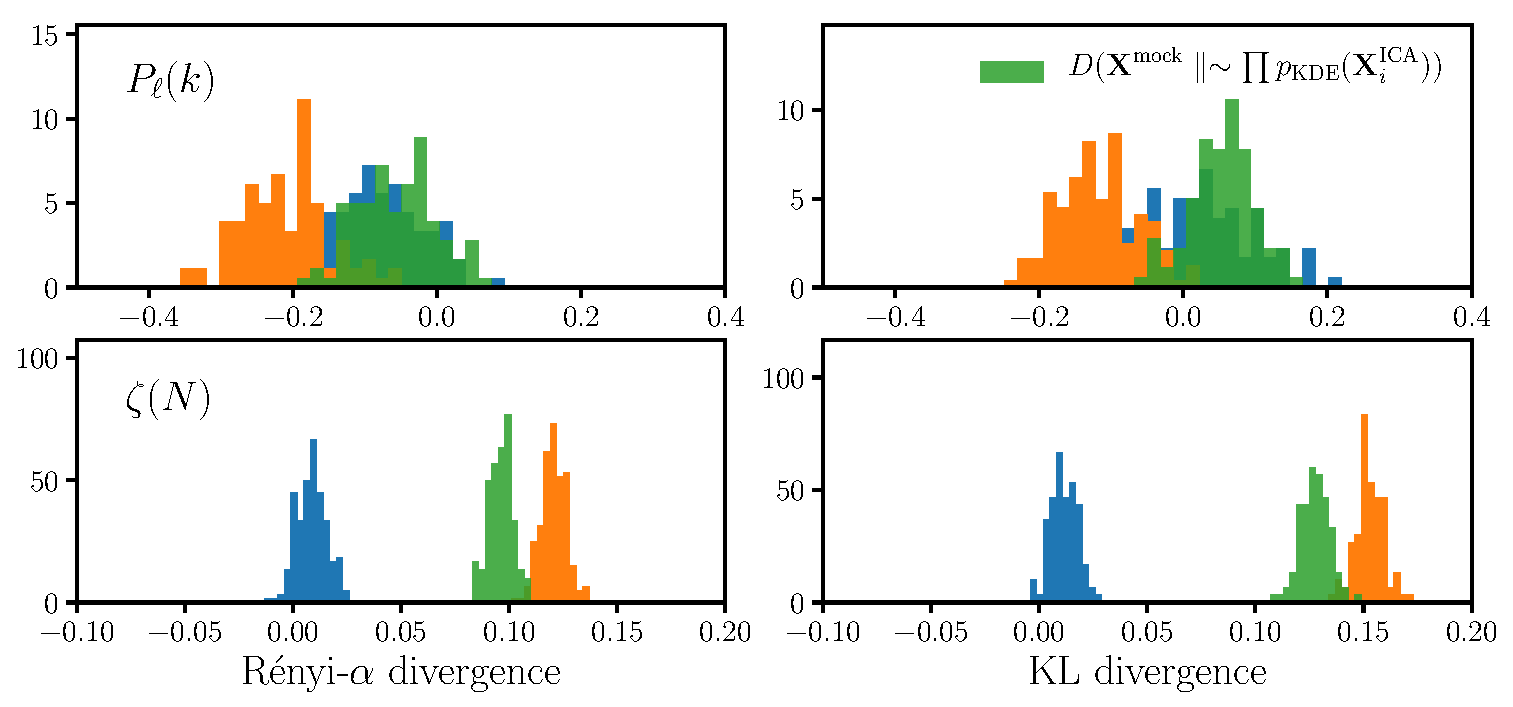
\includegraphics[width=0.9\textwidth]{figs/kNNdiverg_ica.pdf}
\caption{}
\label{fig:div_ica}
\end{center}
\end{figure}

\begin{figure}
\begin{center}
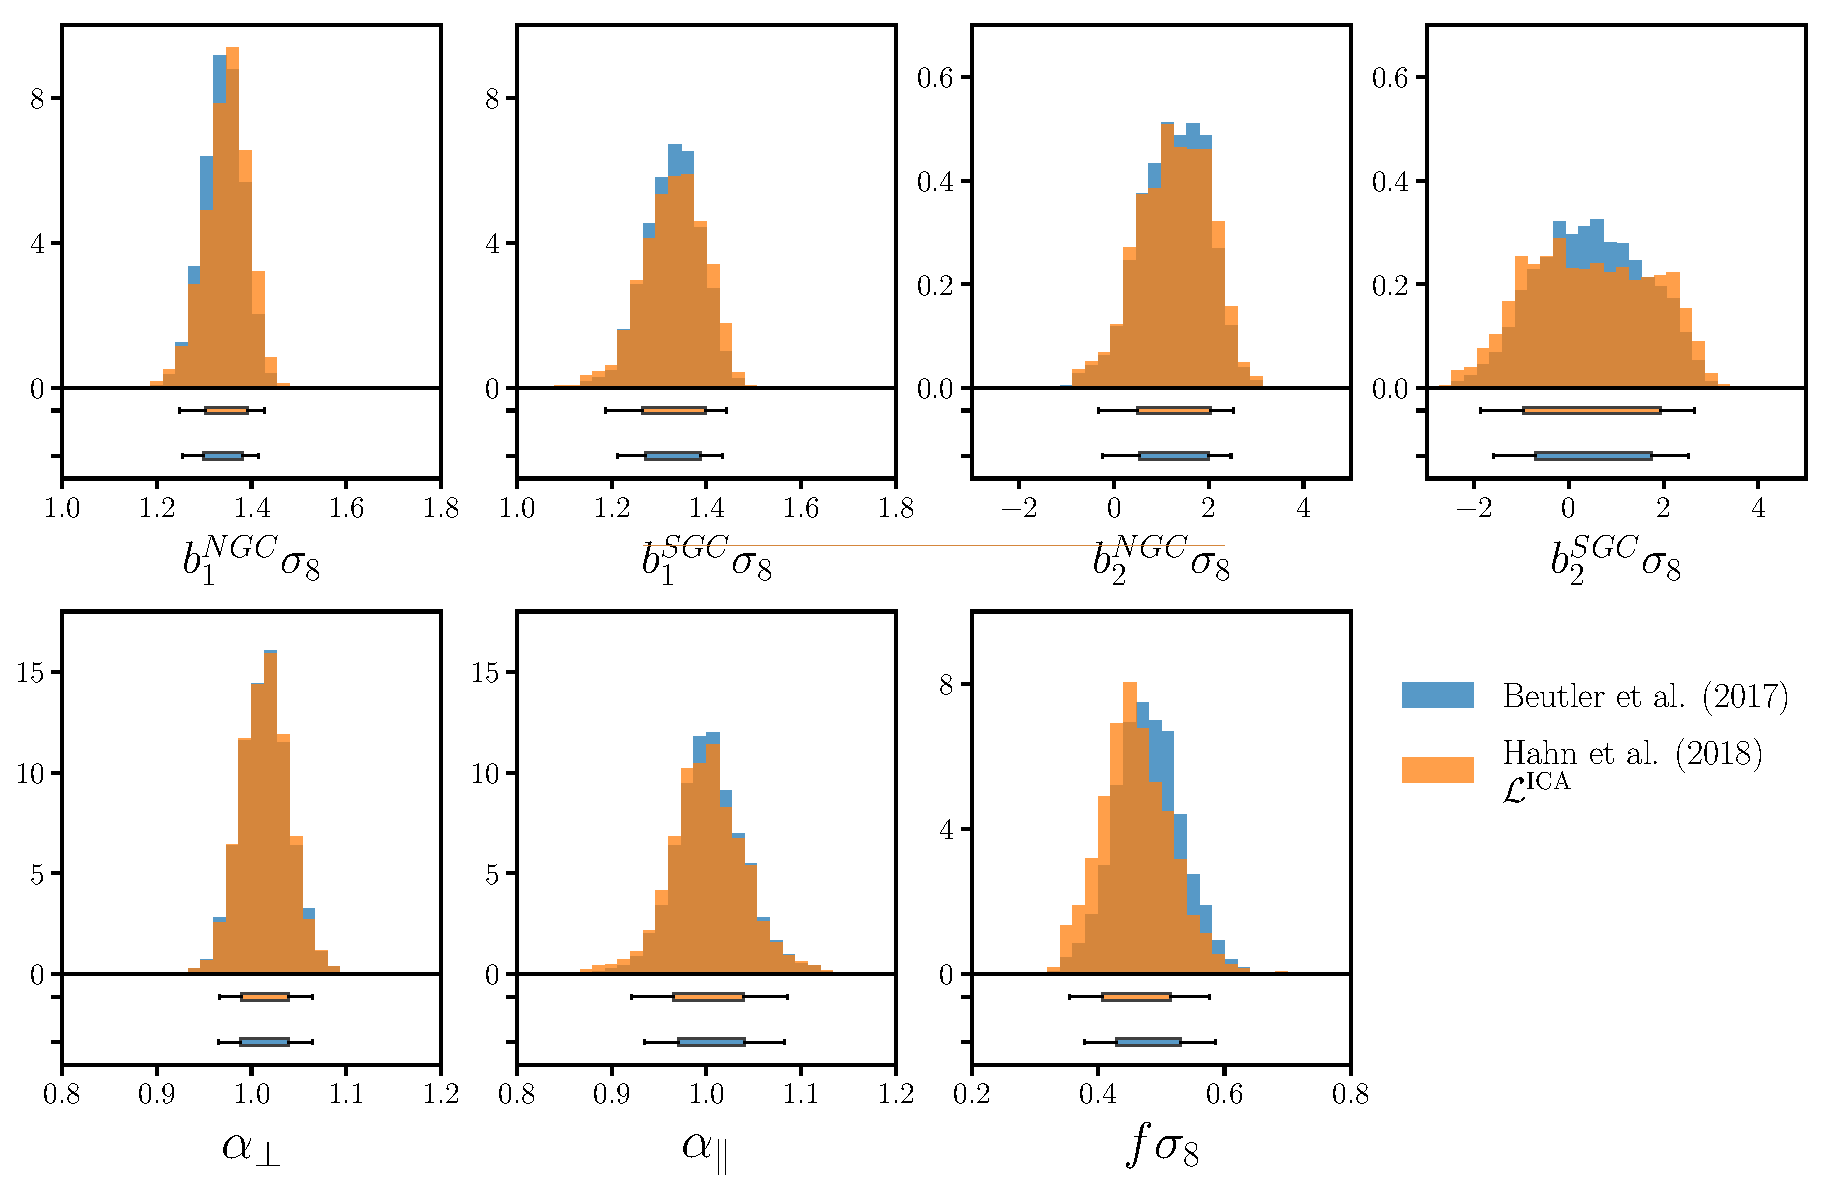
\includegraphics[width=\textwidth]{figs/Like_Pk_comparison.pdf}
\caption{}
\label{fig:pk_like}
\end{center}
\end{figure}

\begin{figure}
\begin{center}
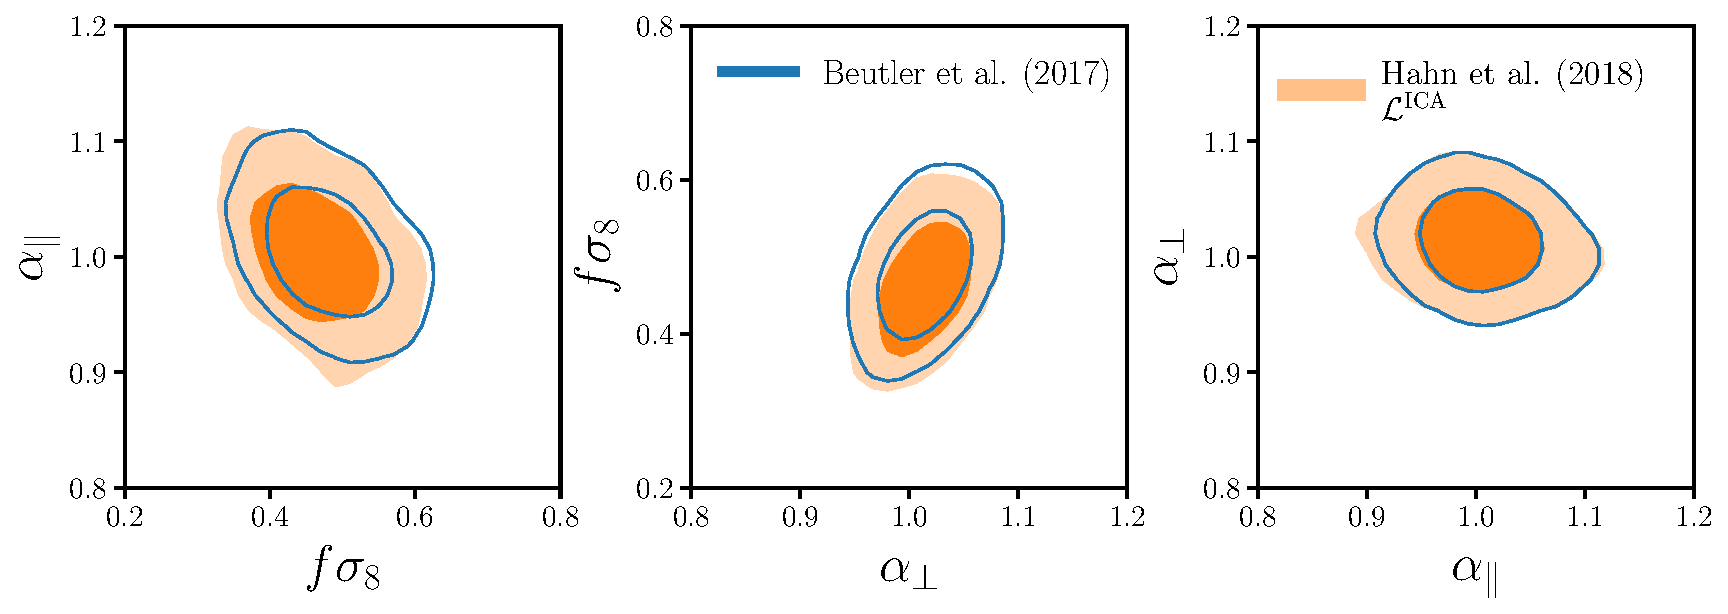
\includegraphics[width=0.9\textwidth]{figs/RSD_contours.pdf}
\caption{}
\label{fig:rsd_contour}
\end{center}
\end{figure}

\begin{figure}
\begin{center}
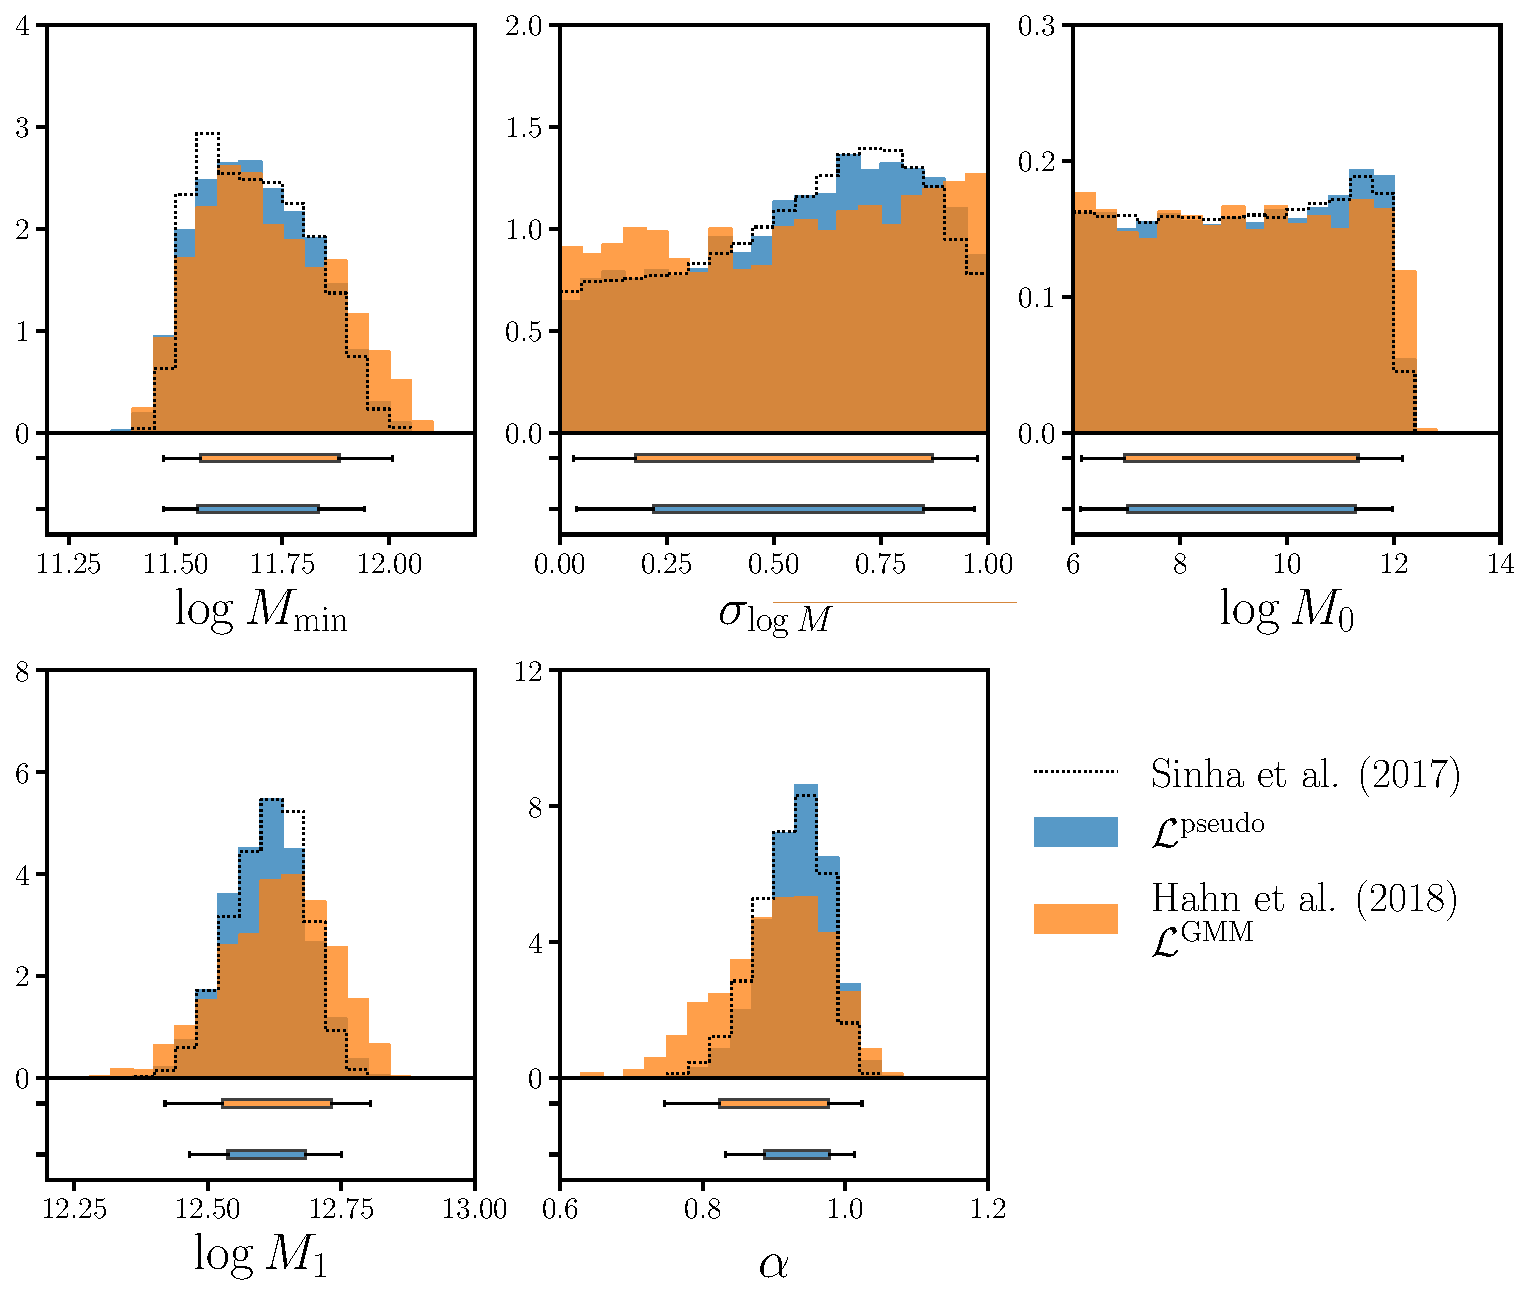
\includegraphics[width=\textwidth]{figs/Like_GMF_comparison.pdf}
\caption{}
\label{fig:gmf_like}
\end{center}
\end{figure}

\begin{figure}
\begin{center}
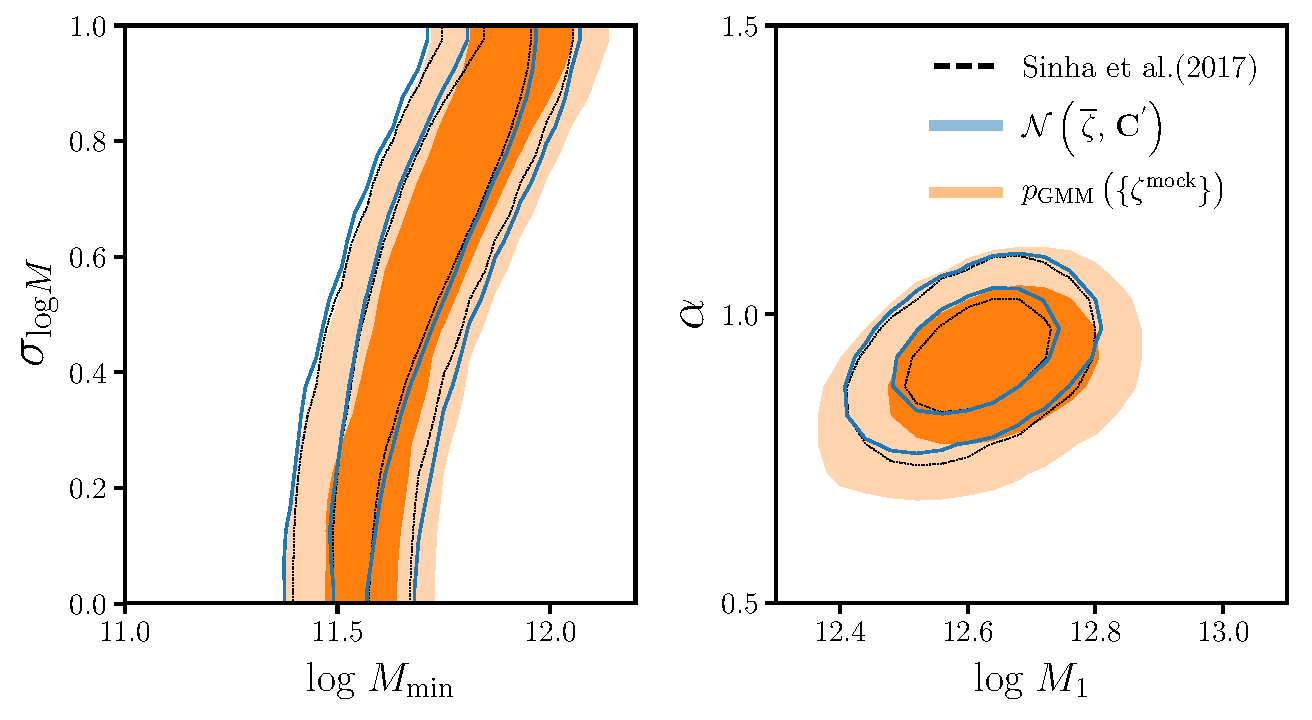
\includegraphics[width=0.8\textwidth]{figs/GMFcontours_manodeep.pdf}
\caption{}
\label{fig:gmf_contour}
\end{center}
\end{figure}

%%%%%%%%%%%%%%%%%%%%%%%%%%%%%%%%%%%%%%%%%%%%%%%%%%%%%%%%%%%%%%%
% Acknowledgements
%%%%%%%%%%%%%%%%%%%%%%%%%%%%%%%%%%%%%%%%%%%%%%%%%%%%%%%%%%%%%%%
\section*{Acknowledgements}
It's a pleasure to thank 
    Simone~Ferraro,
    David~W.~Hogg,
    Emmaneul~Schaan, 
    Roman~Scoccimarro
    Zachary~Slepian

\bibliographystyle{yahapj}
\bibliography{nongausslike}
\end{document}
